
\section{Implementation}

\dejavu{} is implemented in \scalalang{}.   
\dejavu{} takes as input a specification file containing one  or 
more  properties, and synthesizes the monitor as a self-contained \scalalang{} 
program.
This program takes as input the 
trace file and analyzes it.
The tool uses the JavaBDD library for BDD manipulations \cite{javabdd}.

\subsubsection{Example Properties}

Figure \ref{fig:properties} shows three properties in the 
input format of the tool, which are not expressible in the original first-order logic of \dejavu{}. The first property \idsl{telemetry1} is a variant of
formula \ref{eq:wolper-first-order}, illustrating the use of a 
rule to express Wolper's example (\cite{Wolper}) that all the states with even indexes of a sequence satisfy a property.
In this case we consider a radio on board a spacecraft, which communicates over different channels (quantified over in the formula), which can be turned on and off with a \idsl{toggle(x)} - they are initially off.
Telemetry can only be sent to ground over a channel \idsl{x} with the \idsl{telem(x)} event when the radio is toggled on.

\begin{center}
\begin{figure}
\begin{lstlisting}[language=dsl,frame=single,linewidth=0.95\textwidth,backgroundcolor=\color{white},linewidth=\columnwidth,breaklines=true,basicstyle=\small]
prop telemetry1: 
  Forall x . closed(x) -> !telem(x)
  where closed(x) := toggle(x) <-> @!closed(x)

prop telemetry2: 
  Forall x . closed(x) -> !telem(x)
  where
    closed(x) :=
        (!@true & !toggle(x))
      | (@closed(x) & !toggle(x))
      | (@open(x) & toggle(x)),
    open(x) :=
        (@open(x) & !toggle(x))
      | (@closed(x) & toggle(x))

prop spawning : 
  Forall x . Forall y .
  spawn(x,y) -> 
    (P main(x) | Exists z . (P main(z) & leadsto(z,y)))
  where
    leadsto(z,y) := 
        spawn(z,y) 
      | @ leadsto(z,y) 
      | Exists x . (@leadsto(z,x) & spawn(x,y))
\end{lstlisting}
\caption{Three properties stated in \dejavu's logic}
\label{fig:properties}
\end{figure}
\end{center}

The second property, \idsl{telemetry2}, expresses the same 
property as \idsl{telemetry1}, but in this case using two 
rules, more closely reflecting how we would model this using a state machine with two states for each channel \idsl{x}: 
\idsl{closed(x)} and \idsl{open(x)}. The rule \idsl{closed(x)} is defined as a disjunction between three alternatives. The first states that this predicate is true if we are in the initial state 
(the only state where \idsl{@true} is false), and there is no \idsl{toggle(x)} event. The next alternative states that
if \idsl{closed(x)} was true in the previous state and there is
no \idsl{toggle(x)} event, we stay in the \idsl{closed(x)} state.
The third alternative states that if we in the previous state were
in the \idsl{open(x)} state and we observe a \idsl{toggle(x)} event, we transition to the \idsl{closed(x)} state. Similarly for the \idsl{open(x)} rule.

The third property, \idsl{spawning}, expresses a property
about threads being spawned in an operating system. We want to 
ensure that all threads are spawned by the main program or are spawned by a thread that transitively can be traced back to a thread being spawned by the main program. The events are
\idsl{main(x)} (the main program spawns thread \idsl{x}) and
\idsl{spawn(x,y)} (thread \idsl{x} spawns thread \idsl{y}).
For this we need to compute a transitive closure of spawning relationships, here expressed with the rule \idsl{leadsto(z,y)}.

\subsubsection{Monitor Synthesis}

Consider the first \idsl{telemetry1} property. The property-specific 
part\footnote{An additional 600+ lines of property independent 
boilerplate code is generated.} of the synthesized monitor, is shown 
in Figure \ref{fig:monitor}. This function is called for each new event. The function operates on the two arrays holding BDDs, indexed by subformula indexes: \iscala{pre} for the previous state and \iscala{now} for the current state. For each observed event, the function \iscala{evaluate()} computes the \iscala{now} array, evaluating any sub-formula before any formula containing it,
and returns true (property is satisfied in this position of the trace)  iff \idsl{now(0)} is not $\bfalse$. 

\begin{figure}
%\centering
\begin{center}
\begin{tabular}{c}
\begin{lstlisting}[language=scala,basicstyle=\small\sffamily]
override def evaluate(): Boolean = {
  // event nodes:
  now(4) = build("telem")(V("x"))
  now(6) = build("toggle")(V("x"))
  // rule nodes not below @:
  now(7) = pre(8)
  now(5) = now(6).biimp(now(7))
  // rule calls:
  now(2) = now(5)
  now(9) = now(5)
  // rest of rules below @:
  now(8) = now(9).not()
  // rest of main formula:
  now(3) = now(4).not()
  now(1) = now(2).not().or(now(3))
  now(0) = now(1).forAll(var_x.quantvar)

  val error = now(0).isZero
  if (error) monitor.recordResult()
  tmp = now; now = pre; pre = tmp
  !error
}
\end{lstlisting}
\end{tabular}
\end{center}
\caption{Monitor evaluation function for telemetry1}
\label{fig:monitor}
\end{figure}

\begin{figure}
\centering
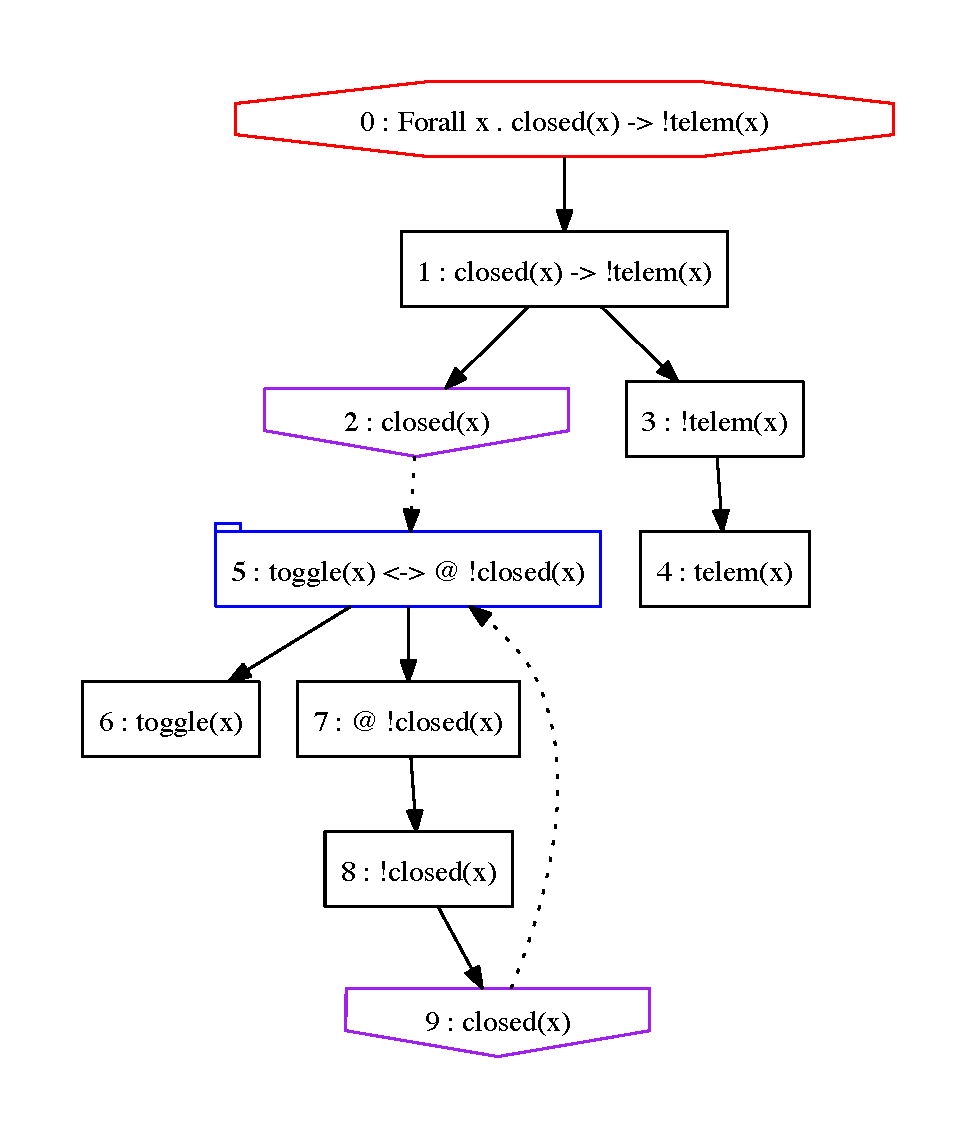
\includegraphics[width=7cm]{figures/ast.pdf}
\caption{Annotated abstract syntax tree for telemetry1}
\label{fig:ast}
\end{figure}

The indexing scheme is guided by an enumeration of the annotated abstract syntax tree of the formula, shown in Figure \ref{fig:ast}. The tree has been annotated by pointing out (blue node 5) the rule body and calls to the rule (purple nodes 2 and 9).
The assignments are evaluated in five steps. First the leaf nodes corresponding to events (4 and 6). Then rule nodes not below the previous-operator \idsl{@} (7 and 5). Then calls of rules (2 and 9)
which can now be calculated since the rule bodies have been calculated. Then the rest of the rules below \idsl{@}  (8). Finally the rest of the main formula (3, 1, 0). At composite subformula nodes, BDD operators are applied. For example for subformula  1, the new  value is \iscala{now(2).not().or(now(3))}, 
which is the interpretation of the formula 
\idsl{closed(x) -> !telem(x)} corresponding to the Boolean law:
$p \rightarrow q = \neg p \vee q$.

\subsubsection{Example Execution}

As an example of how a trace is processed consider the following simple (correct) trace containing two events, turning on low and high frequency channels:
$\mathit{toggle}(``low").\mathit{toggle}(``high")$. The value $``low"$ is assigned the binary enumeration $110$ in node 6, shown in Figure \ref{fig:bdd1}. A dashed line leaving a node means the node has value 0, and a fully drawn line means it has value 1. The BDD represents all assignments to the bit positions 0, 1 and 2 that lead to 1 (shaded square leaf node), in this case 110, read from left to right. Likewise, Figure \ref{fig:bdd2} shows the BBD assigned to node 6 for the second value $``high"$, corresponding to the enumeration 101. Finally Figure \ref{fig:bdd3} shows the BDD representing the rule \idsl{closed(x)} in node 5 after the two events. Since channels $``low"$ and $``high"$, corresponding to enumerations 110 and 101, are now open, this BDD represents all other enumerations. That is, all enumerations except 110 and 110 lead to 1 in this BDD.

\begin{figure}
    \centering   
    \begin{subfigure}[b]{0.15\textwidth}
        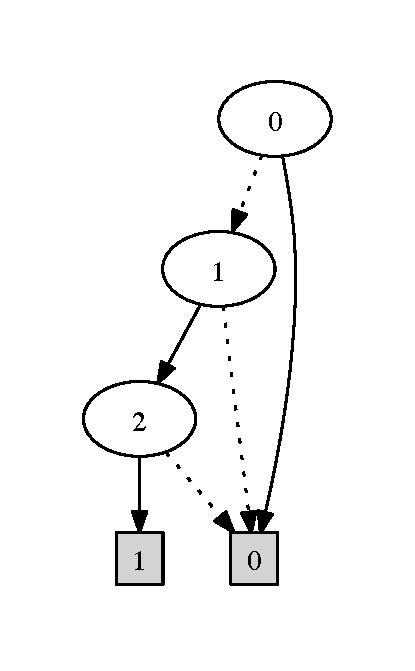
\includegraphics[width=\textwidth]{figures/bdd1.pdf}
        \caption{toggle(``low'')}
        \label{fig:bdd1}
    \end{subfigure}
    ~ 
    \begin{subfigure}[b]{0.15\textwidth}
        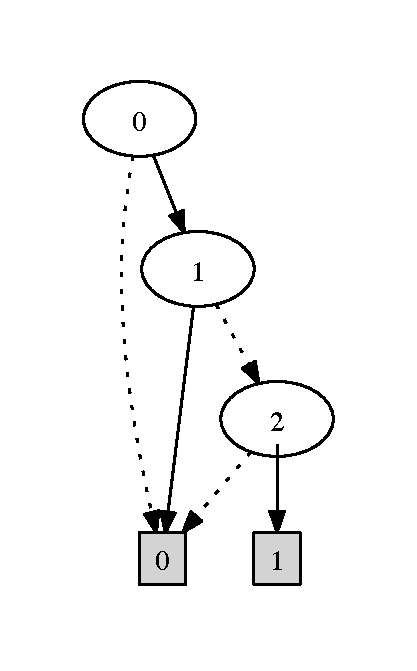
\includegraphics[width=\textwidth]{figures/bdd2.pdf}
        \caption{toggle(``high'')}
        \label{fig:bdd2}
    \end{subfigure}
    ~ 
    \begin{subfigure}[b]{0.15\textwidth}
        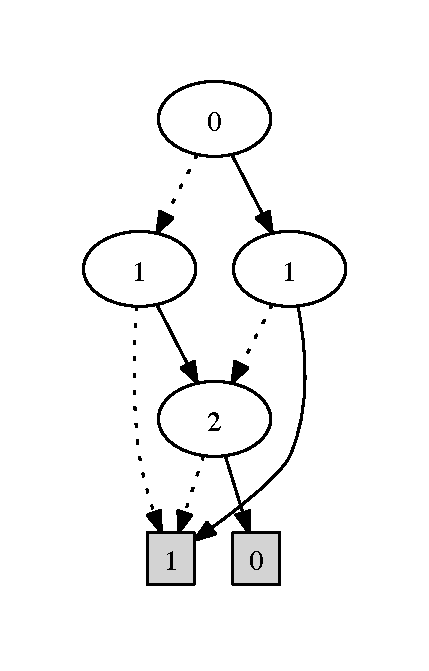
\includegraphics[width=\textwidth]{figures/bdd3.pdf}
        \caption{closed(x)}
        \label{fig:bdd3}
    \end{subfigure}
    \caption{Selected BDDs from trace evaluation}
    \label{fig:bdds}
\end{figure}

\subsubsection{Evaluation}

We evaluated the three properties in Figure 
\ref{fig:properties}. Table \ref{tab:evaluation} shows the  
analysis time (excluding time to compile the generated 
monitor) for different traces (format is `trace length : seconds'). The telemetry traces will repeatedly open hundreds of channels and send telemetry over them, and the spawning traces will spawn a new thread for each event in the trace. The transitive closure of the spawning property needs to process these, therefore the more extensive processing time.

\ignore{
  // repeat: repeat the following
  // repeat_toggle: open this many channels
  // repeat_telem: send this many messages on each channel
}

\ignore{
  // threads: how many threads initially spawned by main program
  // repeat: how many times new threads from new threads are spawned
  // number of spawned threads correspond to number of events
}

\begin{table}[h!]
\centering
\begin{tabular}{|l|c|c|c|}
\hline
Property   & Trace 1 & Trace 2 & Trace 3 \\
\hline
telemetry1 & 1,200,001\,:\,3.3s & 5,200,001\,:\,7.1s & 10,200,001\,:\,12.8s \\
\hline
telemetry2 & 1,200,001\,:\,4.4s & 5,200,001\,:\,9.9s & 10,200,001\,:\,17.9s \\
\hline
spawning   & 4,950\,:\,9.4s & 10,000\,:\,88.4s & 19,900\,:\,488.8s \\
\hline
\end{tabular}
\caption{Evaluation}
\label{tab:evaluation}
\end{table}


